\documentclass{beamer}
%\usepackage{BOONDOX-cal}

\usetheme[progressbar=frametitle]{metropolis}
\setbeamertemplate{frame numbering}[fraction]
\useoutertheme{metropolis}
\useinnertheme{metropolis}
\usefonttheme{metropolis}
\usecolortheme{spruce}
\setbeamercolor{background canvas}{bg=white}

\definecolor{mygreen}{rgb}{.125,.5,.25}
%\usecolortheme{crane}
\usecolortheme[named=mygreen]{structure}
\title{Self Supervised Learning}
\subtitle{Bird Images Clustering}
\author{Phiphat Chomchit}
\institute{CMU}

\date{}
\begin{document}
% Fill color in block
\metroset{block=fill}
	\begin{frame}
		\titlepage
	\end{frame}

	\begin{frame}[t]{Self Supervised Learning?}\vspace{10pt}
	 
		Contrastive self-supervised learning has outperformed supervised pretraining on many downstream tasks like segmentation and object detection.
		
		What if we can get labels for free for unlabelled data and train unsupervised dataset in a supervised manner? We can achieve this by framing a supervised learning task in a special form to predict only a subset of information using the rest. In this way, all the information needed, both inputs and labels, has been provided. This is known as self-supervised learning.
	
	\end{frame}
	
	\begin{frame}[t]{How it work?}\vspace{4pt}
		\begin{figure}
			\centering
			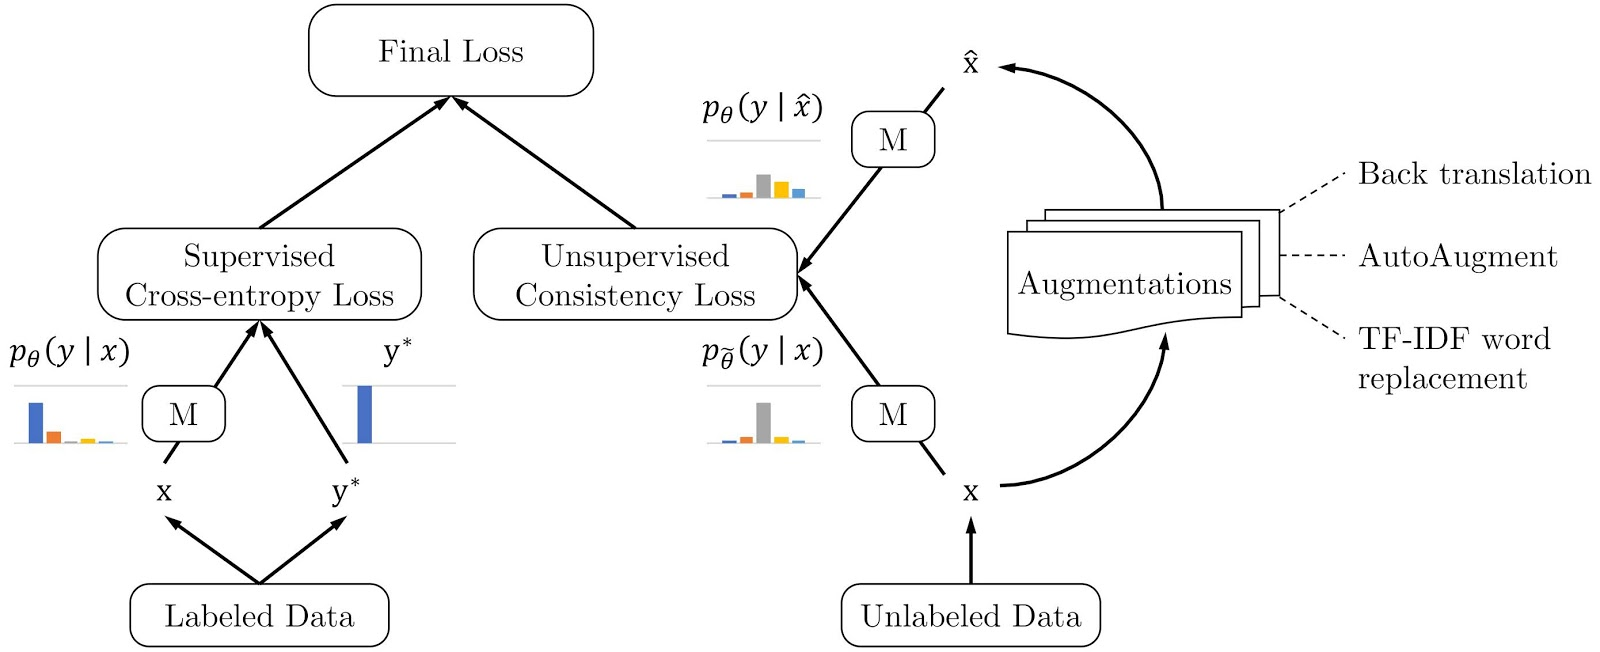
\includegraphics[scale=0.2]{google_semi.jpg}
		\end{figure}
	\end{frame}
	\begin{frame}[t]{Data Augmentation}
	\begin{enumerate}
		\item Colorization
		\item Placing image patches in the right place
		\item Inpainting
	\end{enumerate}
	\end{frame}
	
	\begin{frame}{Colorization}\vspace{4pt}
		 \begin{figure}
		 	\centering
		 	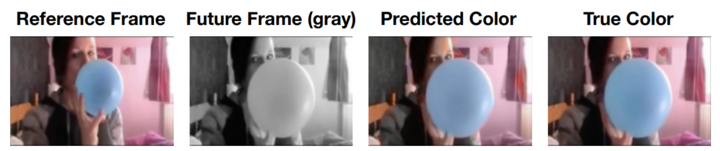
\includegraphics[scale=1]{color.png}
		 \end{figure}
	\end{frame}

	\begin{frame}{Placing image patches in the right place}\vspace{4pt}
		\begin{figure}
			\centering
			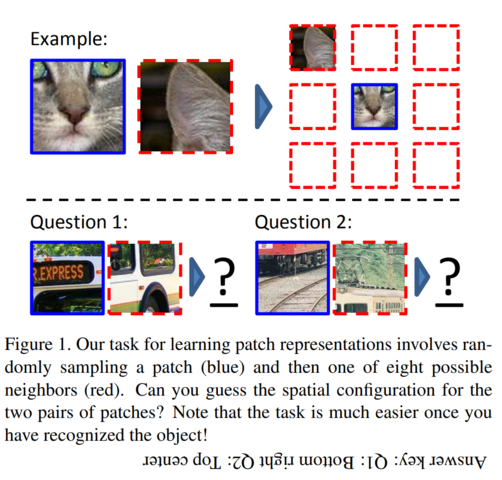
\includegraphics[scale=1]{placing.png}
		\end{figure}
	\end{frame}

	\begin{frame}{Inpainting}\vspace{4pt}
		\begin{figure}
			\centering
			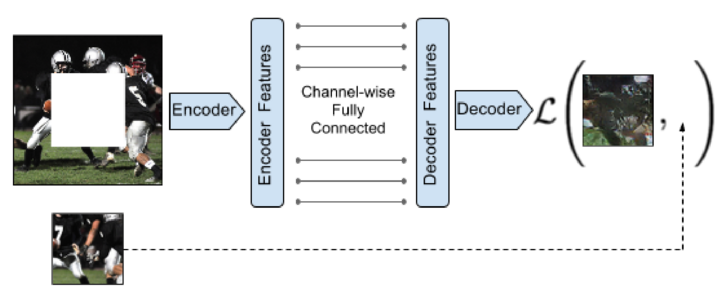
\includegraphics[scale=1]{inpainting.png}
		\end{figure}
	\end{frame}

	\begin{frame}{Method}
		\begin{figure}
			\centering
			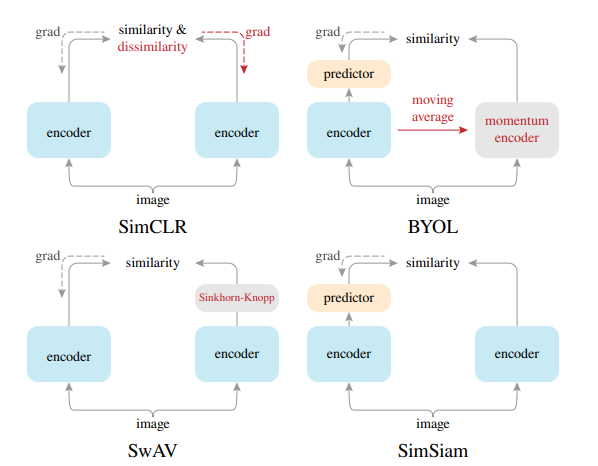
\includegraphics[scale=0.5]{method.png}
		\end{figure}
	\end{frame}
	
	\begin{frame}[t]{Fomulation}
		$$\mathcal{L}(\theta, \eta) = \mathbb{E}_{x, \mathcal{T}}\Big[\|\mathcal{F}_\theta(\mathcal{T}(x)) - \eta_x\|_2^2\Big]$$
		$$\underset{\theta, \eta}{\text{min }} \mathcal{L}(\theta, \eta)$$
		\begin{enumerate}
			\item $\mathcal{F}$ is a network parameterized by $\theta$.
			\item $\mathcal{T}$ is the augmentation.
			\item $x$ is an image.
			\item The expectation $\mathbb{E}[\cdot]$ is over the distribution
			of images and augmentations. For the ease of analysis, here
			we use the mean squared error $\|\cdot\|^2_2$
			\item $\eta_x$ is the representation of the image $x$

		\end{enumerate}
	\end{frame}

	\begin{frame}[t]{Clustering Image with Self-Supervised Learning (Birds)}
		\begin{figure}
			\centering
			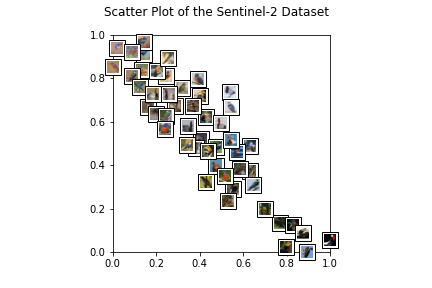
\includegraphics[scale=0.7]{birds.png}
		\end{figure}
	\end{frame}
	
	\begin{frame}[t]{Clustering Image with Self-Supervised Learning (Lands)}
		\begin{figure}
			\centering
			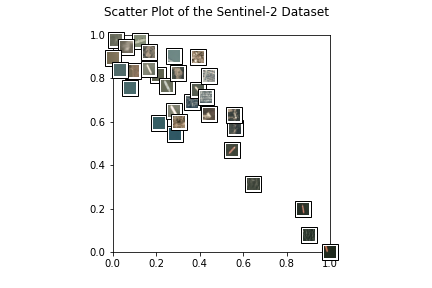
\includegraphics[scale=0.7]{land.png}
		\end{figure}
	\end{frame}

	\begin{frame}[t]{Solution (Birds)}
		\begin{figure}
			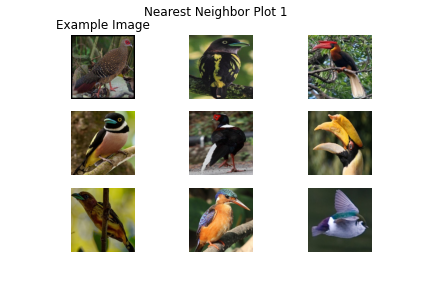
\includegraphics[scale=0.2]{birds0.png}
			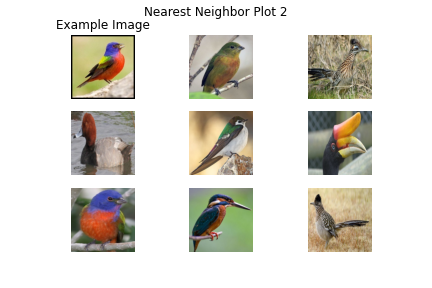
\includegraphics[scale=0.2]{birds1.png}
			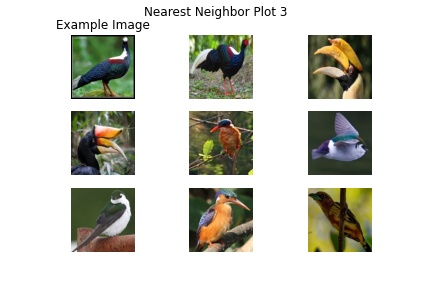
\includegraphics[scale=0.2]{birds2.png}
			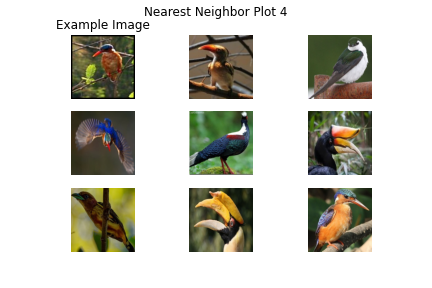
\includegraphics[scale=0.2]{birds3.png}
			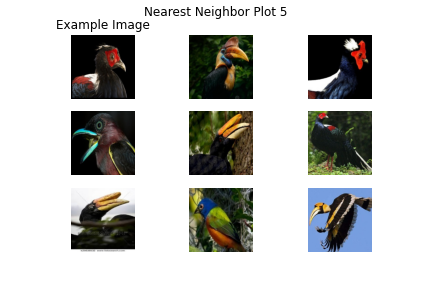
\includegraphics[scale=0.2]{birds4.png}
			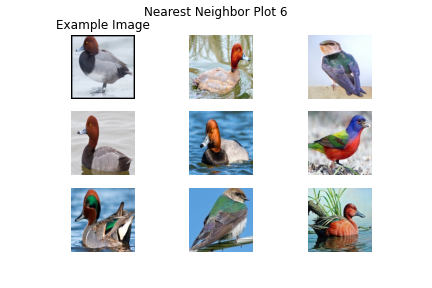
\includegraphics[scale=0.2]{birds5.png}
		\end{figure}
		\end{frame}
	
	\begin{frame}[t]{Solution (Lands)}
		\begin{figure}
			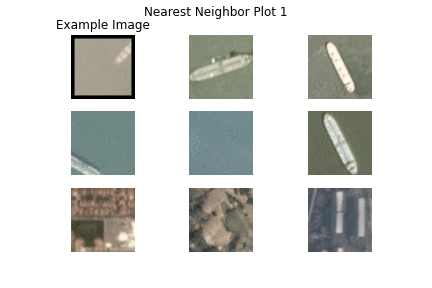
\includegraphics[scale=0.2]{land0.png}
			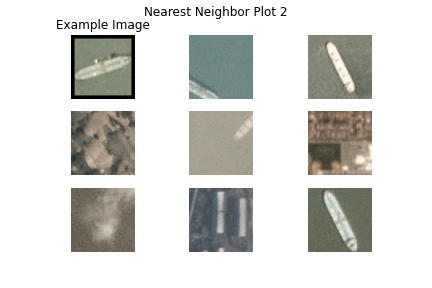
\includegraphics[scale=0.2]{land1.png}
			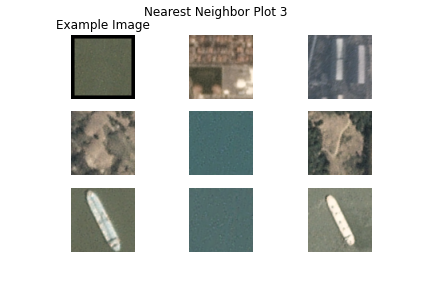
\includegraphics[scale=0.2]{land2.png}
			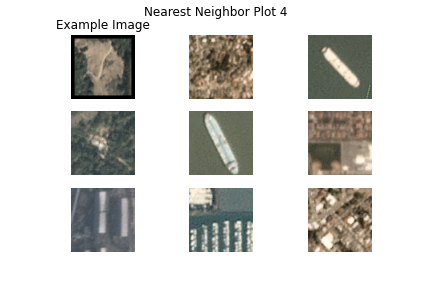
\includegraphics[scale=0.2]{land3.png}
			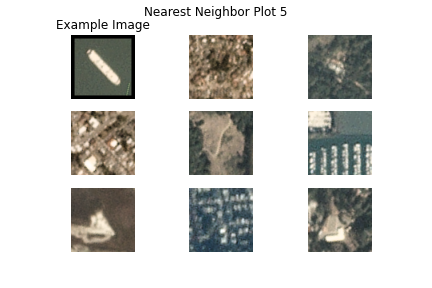
\includegraphics[scale=0.2]{land4.png}
		\end{figure}
	\end{frame}
	\begin{frame}{Any Quation?}
		\begin{figure}
			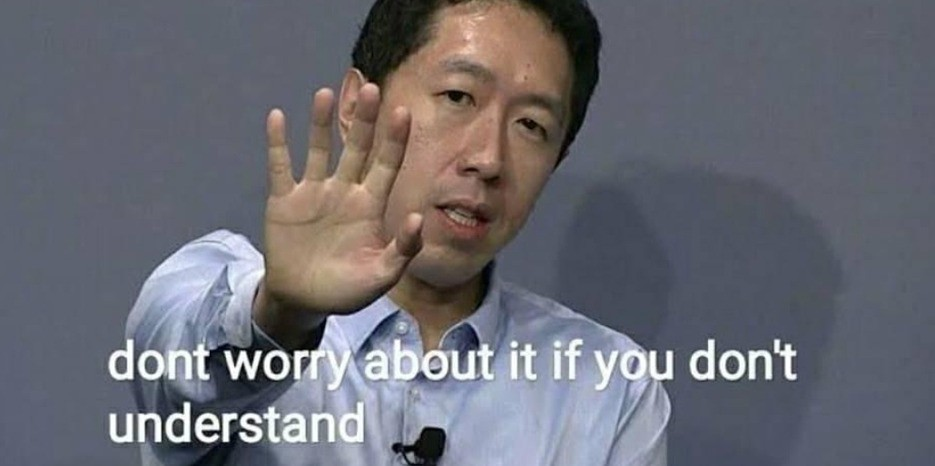
\includegraphics[scale=0.3]{ng.jpg}
		\end{figure}
	\end{frame}

	
	\begin{frame}[standout]
		Thnk you!
	\end{frame}
\end{document}